\documentclass[11pt]{article}
\usepackage{graphicx}
\usepackage{titling}
\usepackage{fancyhdr}
\usepackage[utf8x]{inputenc}
\usepackage{textcomp}
\usepackage{enumerate}
\usepackage{float}
\usepackage{latexsym}
\usepackage{amssymb}
\usepackage{amsthm}
\usepackage{amsfonts}
\usepackage{amsmath}
\usepackage[labelfont=bf]{caption}
\usepackage[usenames,dvipsnames,svgnames,table]{xcolor}
\usepackage{listings}
\usepackage{geometry}
\usepackage{fancyref}
\usepackage{hyperref}
\usepackage{framed}
\usepackage[hypcap]{caption}
\usepackage[toc,page]{appendix}
\parindent=0pt
\frenchspacing

\pagestyle{fancy}

\newcommand{\pctlrepeat}[1]{{\buildrel{#1}\over\curvearrowleft}}
\newcommand{\tbox}[1] {\begin{tabular}{| c |}\hline {#1} \\ \hline\end{tabular}}


\fancyhead[L]{\slshape\footnotesize May 12, 2014\\\textsc{02180 Introduction to Artificial Intelligence}}
\fancyhead[R]{\slshape\footnotesize \textsc{Andreas Kjeldsen (s092638)}\\\textsc{Morten Eskesen (s133304)}}
\fancyfoot[C]{\thepage}

\lstdefinestyle{logoutput}{
	backgroundcolor=\color[RGB]{248,248,248},
	tabsize=1,
	captionpos=b
  	belowcaptionskip=1\baselineskip,
  	breaklines=true,
  	frame=single,
	language={},
  	basicstyle=\footnotesize\ttfamily\color{Black},
	mathescape
}
\newcommand{\tab}{\hspace*{2em}}
\newcommand{\HRule}{\rule{\linewidth}{0.5mm}}

\begin{document}

\begin{titlepage}
\begin{center}


\includegraphics[scale=2.0]{GFX/dtu_logo.pdf}\\[1cm]

\textsc{\LARGE Technical University of Denmark}\\[1cm]

\textsc{\Large 02180 Introduction to Artificial Intelligence 2014}\\[0.5cm]


% Title
\HRule \\[0.4cm]
{\huge \bfseries Heureka Project}\\[0.1cm]
\HRule \\[0.4cm]

% Author and supervisor
\large
\emph{Authors:}
\\[10pt]
Andreas Hallberg \textsc{Kjeldsen}\\
\emph{s092638@student.dtu.dk}
\\[10pt]
Morten Chabert \textsc{Eskesen}\\
\emph{s133304@student.dtu.dk}\\[0.8cm]

{\large May 12, 2014}\\[1.25cm]
\end{center}

\begin{center}
	\textbf{Abstract}
\end{center}
The Heureka Project focuses on graph searching and logical deduction. In this report we will show how to encode data sets for both a map and a knowledge base as directed graphs. Further we will introduce search algorithms for the different data sets, while also describing the heuristics used. We will describe how we optimize our knowledge base and make sure it is consistent. At last we will reflect upon our work, concluding what works and what can be improved.


\end{titlepage}

\section{Introduction}
\label{sec:intro}
This report will focus on our work on the \emph{Heureka Project}, given as an assignment in the DTU course \emph{02180 Introduction to Artificial Intelligence}. The Heureka Project focuses on graph searching, logical deduction and the heuristics.

\subsection{Objectives}
The two objectives for the project are:
\begin{enumerate}
	\item[] \textbf{Route Planning}\\
	Be able to find a route from one point to another point within a map.
	
	\item[] \textbf{Logical Deduction}\\
	Be able to deduce whether a query is satisfied using a knowledge base, either as a direct proof or as a refutation proof. 
\end{enumerate}

\section{Data Representation}
To solve both objectives, we decided to represent our data as graphs. The reasoning behinds this decision, is that a graph can both represent a map and a knowledge base.

\subsection{Map}
For the route planning problem, we are expecting a source file containing the map data. The source file is read and interpreted, generating a directed graph representing the map. Each node represents a coordinate pair {\tt (X, Y)} indicating either a crossing of two streets or an end of a street. Each edge has a name, a weight and represents a partial street. Edge names are not unique, as a street can consist of multiple edges.

\subsubsection{Source File}
The source file should be in plaintext, have one entry per line and use the following syntax:
\begin{itemize}
	\item \tbox{\tt X1 Y1 StreetName X2 Y2}\\
	Where {\tt (X1, Y1)} and {\tt (X2, Y2)} are node coordinates and {\tt StreetName} is the edge name. The weight of the edge is then calculated as the straight line distance from {\tt (X1, Y1)} to {\tt (X2, Y2)}.
\end{itemize}

\subsection{Knowledge Base}
For the logical deduction problem, we are expecting a source file containing the knowledge base. The source file is read and interpreted, generating a directed graph representing the knowledge base.

\subsubsection{Source File}
The source file should be in plaintext, have one entry per line and use one of the following syntaxes:
\begin{itemize}
	\item \tbox{\tt Literal}\\
	Where {\tt Literal} is the ID of the literal. When a literal is stated alone, it is interpreted as being a fact and always satisfiable.
	
	\item \tbox{\tt Literal$_1$ if Literal$_2$ [ $\ldots$ Literal$_n$]}\\
	Where {\tt Literal$_1$, Literal$_2$ $\ldots$ Literal$_n$} are the IDs of the literals. {\tt Literal$_1$} is satisfied if {\tt Literal$_2$ $\ldots$ Literal$_n$} are satisfied. There must be at least one literal to depend on, there is no specific upper limit.
	
	\item \tbox{\tt Literal$_1$ Literal$_2$  [ $\ldots$ Literal$_n$]}\\
	Where {\tt Literal$_1$, Literal$_2$ $\ldots$ Literal$_n$} are the IDs of the literals. Literals listed this way, are being interpreted as a disjunction of the literals. There must be listed at least two literals.
\end{itemize}

Literals can be stated as negative by prepending their ID with a {\tt !}, example:\\ \tbox{\tt !Literal$_1$ if Literal$_2$ !Literal$_3$}

\subsubsection{Nodes}
In the knowledge base, nodes can represent different objects:
\begin{description}
	\item[Literal] Literals are what the knowledge base works with. Literals can be {\tt Positive} and {\tt Negative}, they have a unique ID. A negative literal has a {\tt !} prepended to its ID, which means literal {\tt lit} is a positive literal and literal {\tt !lit} is a negative literal. Literals can be stated as facts, if the positive literal is a fact, the negative literal cannot be, as this would make the knowledge base inconsistent.
	
	\item[Conjunctive Literal] Literals can depend on more than one other literal to be satisfied. In this case we make a node representing the conjunction of the depending literals. The ID of the conjunction will be the IDs of the depending literals in sorted order separated by {\tt \&}. An edge is then made between the literal and the conjunction, and between the conjunction and the literals it represents. If all the literals of a conjunction are facts, then so will the conjunction be.
	
	\item[Disjunctive Literal] In cases where a literal has more than one way to be satisfied, a disjunctive literal can be used. The ID of the disjunction will be the IDs of the literals in sorted order separated by {\tt |}. An edge is made between the literal and the disjunction, and between the disjunction and the literals it represents. If any of the literals in the disjunction are facts, then so will the disjunction be.
\end{description}

The nodes are stored in the graph as either {\tt AND} nodes or {\tt OR} nodes. An {\tt AND} node is satisfied if all nodes it connects to are satisfied. An {\tt OR} node is satisfied if any of the nodes it connects to are satisfied. The scheme for determining the node type is:
$$
\text{Node type} = \begin{cases}
  {\text{\tt AND}} & \text{if {\tt Negative} or {\tt Conjunctive}} \\
  {\text {\tt OR}} & \text{if {\tt Positive} or {\tt Disjunctive}}
\end{cases}
$$

\subsubsection{Edges}
In the knowledge base, edges represent a dependency. If node $n_1$ has an edge to node $n_2$ it indicates that $n_1$ depends on $n_2$.

\subsubsection{Illustration}
View the appendix '\nameref{sec:illustration}' (section \autoref{sec:illustration}), to see an illustration of how the graph looks internally.

\section{Route Planning}
For the route planning problem, we wanted to focus on finding an optimal route according to distance. Our solution does not take speeding limits into considerations nor routes requiring payment (bridges, ferries etc.).

\subsection{Initiating A Search}
To initiate a search, a start node and an end node must be specified. The start and end node are identified by giving two street names and then finding the node corresponding to the crossing of the two streets.

\subsection{Finding A Route}
We chose to use the A* algorithm, with the straight line distance (henceforth \emph{SLD}) as our heuristic function. The SLD heuristic can only be applied if the triangle inequality is satisfied, therefore we assume that the data set supplied satisfies this. Further the SLD heuristic is both admissible and monotonic.\\
\\
The A* algorithm makes use of a priority queue to keep track of which node to expand next. The priority queue prioritizes the nodes based on their score, where their score is the cost of going to the node + the SLD to the goal node. The priority queue should be able to update values, due to the scenario when a node is found multiple times, the best possible score should be used. To support this, we implemented a priority queue using a binary heap supported by a dictionary. This gave us the possibility of making constant time look ups, and decrease value updates by $O(n)$ time.

\subsection{Example Run}
Running our route planner on data set '\nameref{subsec:oneway}' (see \ref{subsec:oneway}), using the corner of {\tt SktPedersStraede} and {\tt Larsbjoernsstraede} as starting point, and the corner of {\tt Studiestraede} and {\tt Larsbjoernsstraede} as ending point, gave the following result:
\begin{lstlisting}[style=logoutput]
SktPedersStraede -> LarslejStraede -> Noerrevoldgade ->
Vestervoldgade -> Studiestraede
\end{lstlisting}

\section{Logical Deduction}
For our inference engine, we wanted to be able to support both direct proofs and indirect proof. Our inference engine uses the \emph{Closed World Assumption} when conducting a proof.

\subsection{Optimizing The Knowledge Base}
Removing unwanted properties of the knowledge base such as inconsistencies and self-evident clauses, while also avoiding duplicate clauses and literals, are ways of optimizing the knowledge base.

\subsubsection{Removing Duplicates}
We chose that the knowledge base should encode a literal as two nodes within our graph, once as a positive literal and once as a negative literal. Whenever a clause is added to our knowledge base, all the literals the clause consists of, are added to the knowledge base, afterwards the dependencies implied by the clause are created by adding edges between the nodes corresponding to the literals. If a literal has already been added, it will not be added again. Encoding our knowledge base this way, ensures that all literals and clauses will only be added once.

\subsubsection{Inconsistency}
When adding a clause to the knowledge base, we check for inconsistency. We determine the knowledge base is inconsistent if:
\begin{itemize}
	\item If both the positive and negative node of a literal are stated as facts.
	\item If both the positive and negative node of a literal can be determined as being a fact based on their dependencies.
	\item If any literal at some point depend on both the positive and negative node of another literal.
\end{itemize}

\subsubsection{Self-evident Clauses}
If the head of a clause is also stated as one of the dependent literals, the head is removed from the dependent literals. Further if the head is depending on its negated self, the clause would never become true, and is therefore invalid.

\subsection{Initiating A Search}
The inference engine can answer queries. We interpret the queries as a conjunction of all the literals listed in the query. A query of {\tt "a b c"} would be interpreted as {\tt "a $\wedge$ b $\wedge$ c"}.

\subsection{Searching For Proof}
A search for a proof is carried out by having a set of start nodes. Our algorithm will then do a \emph{Depth First Search} (henceforth DFS), starting at all the start nodes. Every time a node is reached that is not listed as satisfied and that has not been visited already, a search for proving that literal is initiated. When a node is reached and all of its dependencies (if any) have already been checked and the node is not a fact, its assumed that the literal is not satisfied. The inference engine always answers {\tt true} or {\tt false} to a query, never {\tt unknown/maybe}.

\subsubsection{Direct Proof}
When conducting the direct proof, we start the search at the literals from the query. All the literals have to be satisfied for the query to be satisfied.

\subsubsection{Indirect Proof}
When conducting the indirect proof, we first negate all the literals. Then we start the search at the negated literals. If any of the negated literals are satisfied, the query is not satisfied, otherwise the query is assumed to be satisfied. This can sometimes lead to false positives, as an example querying the knowledge base build from the data set '\nameref{subsec:inconsamp}' (see \ref{subsec:inconsamp}) for {\tt "a"} would claim that {\tt a} was satisfied, as {\tt !a} isn't satisfied.

\subsubsection{Heuristics}
We do not use any heuristics when performing our search. This is due to several complications we encountered.\\
\\
We wanted to give the nodes coordinates, in such a way that if a node were dependent on another, they were close by. If the nodes had coordinates, that satisfied the triangle inequality we could have used SLD as our heuristic. Unfortunately, we didn't have a proper algorithm for clustering the nodes together, therefore we discarded the idea of using SLD as our heuristic.\\
\\
We also tried to give the edges between the nodes weights, where the weight was equal to the amount of literals in the end node. Using $h(0)$ as our heuristic function in combination with the edge weights, we could use A* for searching. Doing so would make the inference engine prioritize paths that had the least amount of literals to be checked. We did some benchmarking, but it showed that doing a normal DFS instead was at least as fast, as using A*. Therefore we decided not to include any heuristics in our search.

\subsection{Example Run}
Running our inference engine on data set '\nameref{subsec:simplesamp}' (see \ref{subsec:simplesamp}), we get the following results querying for '{\tt q}':
\begin{lstlisting}[style=logoutput]
[Direct] Is q satisfiable?
a is satisfied
a & p is not satisfied
a & b is satisfied
l is satisfied
b is satisfied
b & l is satisfied
m is satisfied
l & m is satisfied
p is satisfied
q is satisfied
[Direct] Yes q is satisfiable

[Refutation] Is q satisfiable?
!a is not satisfied
!a | !p is not satisfied
!l is not satisfied
!b is not satisfied
!b | !l is not satisfied
!m is not satisfied
!l | !m is not satisfied
!p is not satisfied
!q is not satisfied
[Refutation] Yes q is satisfiable
\end{lstlisting}

\section{Conclusion}
We have managed to encode the data sets for both problems as graphs, making it possible to use the same code to solve both problems.

\subsection{Route Planning}
Our route planner works, it's fast and finds an optimal route according to distance. An improvement would be to include speeding limits on the roads, this would make it possible to plan the route according to traveling time instead of distance, or even make a hybrid that would take both into consideration. It would also be advantageous to include bridges, ferries and the like, also stating the cost of using these.

\subsection{Logical Deduction}
Our inference engine can properly answer queries using both direct proof and indirect proof within the closed world assumption. Though we do optimize our knowledge base by removing some redundant clauses and dependencies, there are still ways to optimize it further (removing circular dependencies etc.).\\
\\
The way we're conducting our indirect proof, can sometimes result in false positives, this is not satisfactory but we believe its a quirk. 
\\
\\
We didn't choose to implement our inference engine using heuristics, but putting more research into finding a proper heuristic function would most likely be beneficial.


\clearpage
\pagenumbering{Roman}
\begin{appendices}

\section{Data Sets}
Below are some of the data sets we used for testing.

\subsection{Route Planning}
\subsubsection{One-way Streets}
\label{subsec:oneway}
\lstinputlisting[style=logoutput,inputencoding=utf8x,extendedchars=\true]{../Heureka/TestInputs/pathtestinput01.txt}

\subsection{Logical Deduction}
\subsubsection{Simple Sample}
\label{subsec:simplesamp}
\lstinputlisting[style=logoutput,inputencoding=utf8x,extendedchars=\true]{../Heureka/TestInputs/logic02simple.txt}

\subsubsection{Inconclusive Sample}
\label{subsec:inconsamp}
\lstinputlisting[style=logoutput,inputencoding=utf8x,extendedchars=\true]{../Heureka/TestInputs/logic03simple.txt}

\subsubsection{Breakfast}
\label{subsec:breakfastsamp}
\lstinputlisting[style=logoutput,inputencoding=utf8x,extendedchars=\true]{../Heureka/TestInputs/logic05breakfast.txt}

\clearpage
 
\section{Knowledge Base Illustration}
\label{sec:illustration}
Below is an illustration of the graph used by the knowledge base. The illustration is generated using Graphviz\footnote{Graphviz - Graph Visualization Software:  \url{http://www.graphviz.org/}.}. The shape of the nodes indicate what kind of node they are, rectangular nodes are {\tt AND} nodes, circular nodes are {\tt OR} nodes. The color of the nodes indicate whether or not the nodes are facts, a {\tt grey} or {\tt yellow} node is not known to be a fact, a {\tt blue} or {\tt green} node is known to be a fact.

\subsection{Breakfast Example}
The example below is build upon the data set '\nameref{subsec:breakfastsamp}' (see \ref{subsec:breakfastsamp}).\\
\begin{center}
	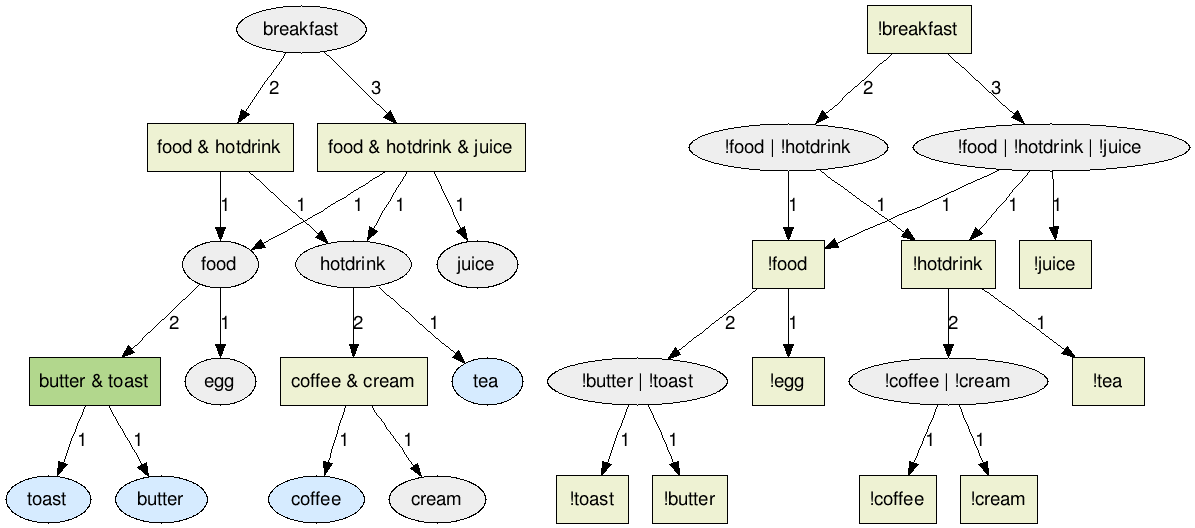
\includegraphics[scale=0.35]{GFX/breakfast_example.png}
\end{center}
\end{appendices}

\end{document}
